% ============================================================
% IEEE conference paper — "Does Compressibility Transfer Across
% Sensors?" — IEEEtran conference template
% (https://www.ieee.org/conferences/publishing/templates)
% Hard limit: 6 pages including references.
% Figure is self-contained (pgfplots) — no image files needed.
% ============================================================
\documentclass[conference]{IEEEtran}
\IEEEoverridecommandlockouts

\usepackage{cite}
\usepackage{amsmath,amssymb,amsfonts}
\usepackage{graphicx}
\usepackage{booktabs}
\usepackage{multirow}
\usepackage{xcolor}
\usepackage{textcomp}
\usepackage{pgfplots}
\pgfplotsset{compat=1.16}
\usepgfplotslibrary{groupplots}
\usetikzlibrary{calc}

\newcommand{\TODO}[1]{\textcolor{red}{[TODO: #1]}}

\begin{document}

\title{Does Compressibility Transfer Across Sensors?\\
A Cross-Dataset Study of CNN Pruning for Optical and SAR Flood
Classification}

\author{\IEEEauthorblockN{Abdul Rauf}
\IEEEauthorblockA{\textit{Faculty of Computer Science and Engineering} \\
\textit{Ghulam Ishaq Khan Institute of Engineering Sciences and Technology}\\
Topi, Pakistan \\
u2024020@giki.edu.pk}
\and
\IEEEauthorblockN{\TODO{supervisor name}}
\IEEEauthorblockA{\textit{\TODO{department}} \\
\textit{\TODO{university}}\\
\TODO{city, country} \\
\TODO{email}}
}

\maketitle

\begin{abstract}
Magnitude pruning is the standard route to deploying convolutional
networks on the resource-constrained platforms used in disaster
response, yet pruning recipes are almost always validated on optical
benchmarks. We ask whether the compressibility of a CNN transfers
across sensing modalities. Under a single fixed supervised pipeline, we
train ResNet18 and VGG-16 flood classifiers on FloodNet (optical UAV
imagery) and Sen1Floods11 (Sentinel-1 SAR, converted from per-pixel
masks to image-level labels), and prune each model with global
unstructured and filter-level structured $L_1$ pruning, fine-tuning
every configuration identically; we report final-epoch accuracy,
balanced accuracy, macro-F1 and AUC as mean~$\pm$~std over three seeds
(96 runs). On these two datasets, unstructured compressibility
transfers: ResNet18 loses at most $0.03$ macro-F1 at 90\% sparsity on
both. Structured pruning does not: at 50\% filter pruning the
FloodNet model loses $0.001$ macro-F1 while the Sen1Floods11 model
loses $0.068$, the gap widens monotonically with ratio, and a lower
fine-tuning learning rate does not close it. VGG-16 is reported as an
instability case: its dense SAR training already fails on one of three
seeds (accuracy swings while AUC remains $0.858$, indicating a
decision-threshold rather than a representation failure), and its
structured variants collapse to constant predictors on both datasets.
Our results indicate that sparsity budgets established on one sensor
cannot be assumed to hold on another, and that compression choices
should be re-validated per dataset and modality.
\end{abstract}

\begin{IEEEkeywords}
network pruning, model compression, flood detection, SAR, optical
remote sensing, FloodNet, Sen1Floods11
\end{IEEEkeywords}

% ------------------------------------------------------------------
\section{Introduction}
Rapid flood mapping is one of the most time-critical applications of
remote sensing: response teams need scene-level situational awareness
within hours of a disaster, often from platforms --- small UAVs, edge
boxes, nanosatellites --- that cannot host large networks
\cite{rahnemoonfar2021floodnet,khan2023floodresnet50}. Model
compression, and in particular magnitude pruning
\cite{han2015learning,li2017pruning}, is the standard route to meeting
such constraints: weights or whole filters with small magnitude are
removed and the network is fine-tuned, frequently recovering accuracy
at high sparsity \cite{blalock2020state}.

The evidence base for this practice, however, is narrow in one
important way. Pruning methods are overwhelmingly validated on optical
(RGB) benchmarks such as ImageNet \cite{deng2009imagenet}, and when
they are applied in remote sensing it is typically to a single dataset
at a time. Flood monitoring in practice spans at least two very
different sensing modalities: high-resolution optical imagery from
UAVs, which is only available in clear conditions, and synthetic
aperture radar (SAR), which penetrates cloud cover and is often the
only usable source during the flood event itself
\cite{bonafilia2020sen1floods11}. A deployment pipeline that
compresses a model for the optical case will sooner or later be asked
to do the same for the SAR case.

This paper is built around a single question:
\begin{quote}
\emph{Does a heavily pruned classic CNN hold its accuracy consistently
on both optical and SAR flood imagery, or does one modality break down
while the other does not?}
\end{quote}
Either answer is informative. If compressibility transfers, then
sparsity budgets established on optical benchmarks can be reused for
SAR deployments with reasonable confidence. If it does not --- if one
dataset degrades earlier or collapses outright --- then the pruning
ratio itself becomes a dataset-dependent hyperparameter, and
compression recipes must be re-validated per sensor and dataset.

Answering the question fairly requires removing every confound except
the data. We therefore fix a single supervised pipeline --- identical
architecture definitions, input resolution, augmentation, class
balancing, optimizer, schedule, evaluation protocol, pruning
operators, sparsity ratios, and fine-tuning budget --- and vary
\emph{only} the dataset. We instantiate the study with two standard
backbones of very different capacity, ResNet18 (11.2M parameters)
\cite{he2016resnet} and VGG-16 (134.3M parameters)
\cite{simonyan2015vgg}, on two public flood-classification datasets:
FloodNet \cite{rahnemoonfar2021floodnet}, optical UAV imagery from
Hurricane Harvey, and Sen1Floods11 \cite{bonafilia2020sen1floods11},
Sentinel-1 SAR chips of global flood events. Sen1Floods11 is labeled
per pixel, so we convert its hand-labeled water masks into image-level
flooded/non-flooded labels with an explicit, reproducible rule
(Section~\ref{sec:setup}).

\noindent\textbf{Contributions.}
\begin{itemize}
\item A controlled cross-dataset pruning study (two architectures, two
datasets, two pruning families, multiple sparsity ratios, three seeds;
96 trained models) in which the training pipeline is held fixed and
only the dataset varies.
\item A reproducible protocol for converting per-pixel SAR flood masks
(Sen1Floods11) into image-level classification labels, enabling
like-for-like comparison with image-level optical benchmarks
(FloodNet).
\item Evidence that, on these two datasets, compressibility under
\emph{unstructured} pruning transfers (ResNet18: $\leq 0.03$ macro-F1
cost at 90\% sparsity on both), whereas \emph{structured} pruning does
not (at 50\%: $-0.001$ macro-F1 on FloodNet vs.\ $-0.068$ on
Sen1Floods11), and that a lower fine-tuning learning rate does not
close the gap --- i.e., the SAR-side drop is not an artifact of our
fine-tuning recipe.
\item An analysis of VGG-16 as an instability case: seed-level failure
of dense SAR training that manifests as a decision-threshold
(final-epoch) problem while AUC stays stable, and layer-level collapse
of its structured variants, which we attribute to the absence of skip
connections.
\end{itemize}

% ------------------------------------------------------------------
\section{Related Work}
\subsection{Flood Classification Datasets and Baselines}
\textbf{FloodNet} \cite{rahnemoonfar2021floodnet} is a high-resolution
($3000\times4000$) UAV imagery dataset collected after Hurricane
Harvey, providing a semi-supervised Track-1 challenge with 398 labeled
training images (51 flooded, 347 non-flooded), 1{,}047 unlabeled
training images, and validation/test splits whose classification
labels were withheld for the challenge evaluation.
\textbf{Sen1Floods11} \cite{bonafilia2020sen1floods11} provides 4{,}831
Sentinel-1 SAR chips of $512\times512$ pixels covering 11 global flood
events, including 446 hand-labeled chips whose per-pixel masks
distinguish water, non-water, and invalid pixels; it is designed for
per-pixel flood segmentation rather than image-level classification,
which motivates the label conversion of Section~\ref{sec:setup}.

On the modeling side, Khose \emph{et al.}
\cite{khose2021semisupervised} established a strong FloodNet Track-1
classification baseline: a ResNet18 trained with pseudo-label
semi-supervision \cite{lee2013pseudo} reaching 96.70\% test accuracy
with 11.6M parameters --- outperforming substantially larger
InceptionV3, ResNet50 and Xception baselines. Their result motivates
our choice of ResNet18 as the small reference backbone; in this work,
however, we deliberately use \emph{purely supervised} training for all
runs, since pseudo-labeling would entangle compression effects with
semi-supervision effects. Closest to our deployment motivation, Khan
\emph{et al.} \cite{khan2023floodresnet50} propose Flood-ResNet50, a
modified ResNet50 for flooded/non-flooded UAV image classification
evaluated on-device (Jetson Nano) with 96.43\% accuracy and 86.36\% F1
on FloodNet. Their study targets efficiency via architecture design on
a single optical dataset; ours is complementary, asking whether a
\emph{given} architecture compressed by pruning behaves consistently
across an optical and a SAR dataset.

\subsection{Network Pruning}
Magnitude pruning removes parameters deemed unimportant by weight
magnitude. \emph{Unstructured} pruning \cite{han2015learning} zeroes
individual weights globally across layers and achieves high sparsity
with little accuracy loss, though realized speedups require sparse
kernels. \emph{Structured} pruning \cite{li2017pruning} removes entire
filters or neurons, producing dense sub-networks that accelerate on
commodity hardware but constraining what can be removed. Subsequent
work has questioned what pruning actually preserves: the lottery-ticket
hypothesis \cite{frankle2019lottery} locates sparse trainable
sub-networks, Liu \emph{et al.} \cite{liu2019rethinking} argue that
the value of pruning lies largely in the architecture it induces, and
Blalock \emph{et al.} \cite{blalock2020state} document that pruning
papers overwhelmingly evaluate on a small set of optical benchmarks
under inconsistent protocols. To our knowledge, no prior work has held
a flood-classification pipeline fixed and measured how the \emph{same}
pruning protocol behaves across an optical and a SAR dataset; this is
the gap we address.

% ------------------------------------------------------------------
\section{Experimental Setup}
\label{sec:setup}

\subsection{Datasets and Label Conversion}
\textbf{FloodNet (optical).} We use the 398 labeled Track-1 training
images (51 flooded / 347 non-flooded). Because classification labels
for the official validation and test splits were withheld for the
challenge server, all labeled evaluation must come from these 398
images: we use a stratified 50/50 split (199 train / 199 validation,
fixed seed), mirroring the split strategy of the public baseline
implementation \cite{khose2021semisupervised}. Images are resized from
$3000\times4000$ to $400\times300$.

\textbf{Sen1Floods11 (SAR).} We use the hand-labeled subset:
Sentinel-1 chips with two polarization bands (VV, VH) and per-pixel
masks with values
$\{1{=}\text{water},\,0{=}\text{non-water},\,-1{=}\text{invalid}\}$.
Since the dataset is natively per-pixel, we convert each chip to an
image-level label with the rule
\begin{equation}
y = \mathbf{1}\!\left[\frac{\left|\{p : m_p = 1\}\right|}
{\left|\{p : m_p \neq -1\}\right|} \;\geq\; \tau\right],
\qquad \tau = 0.01,
\label{eq:labelconv}
\end{equation}
i.e., a chip is \emph{flooded} if at least 1\% of its valid pixels are
water; chips with no valid pixels are discarded. This yields 441
usable chips (293 flooded / 148 non-flooded), split 50/50 stratified
into 220 train / 221 validation chips with the same fixed seed. For
input compatibility with ImageNet-pretrained backbones, SAR
backscatter is clipped to $[-50, 1]$\,dB, min--max scaled to $[0,1]$,
and stacked as three channels $(\mathrm{VV}, \mathrm{VH},
(\mathrm{VV}{+}\mathrm{VH})/2)$, then bilinearly resized to
$400\times300$.

The two datasets are imbalanced in \emph{opposite} directions: flooded
images are the minority class in FloodNet (12.8\%) but the majority
class in Sen1Floods11 (66.4\%). We therefore report balanced accuracy
and macro-F1 alongside accuracy and AUC, and we compare each pruned
model only to its own dense baseline, never across datasets in
absolute terms.

\subsection{Unified Training Pipeline}
All dense baselines and all fine-tuning runs share one pipeline,
identical across datasets and architectures: ImageNet-pretrained
backbone \cite{deng2009imagenet} with the final layer replaced by a
2-logit head; cross-entropy loss; random horizontal and vertical flips
as the only augmentation; a class-balanced weighted random sampler;
SGD with learning rate $0.01$ and no momentum; and 50 epochs. We
deliberately evaluate the \emph{final-epoch} checkpoint --- no
early stopping and no best-validation selection --- so that reported
numbers are not inflated by checkpoint cherry-picking. Each
configuration is run with three seeds (42, 124, 2024) that vary
initialization, sampling and augmentation randomness while the data
split stays fixed; we report mean~$\pm$~std. The only
architecture-forced difference is the batch size (64 for ResNet18, 16
for VGG-16, due to memory at $400\times300$); it is held constant
across datasets so that every FloodNet-vs-Sen1Floods11 comparison is
batch-size matched.

\subsection{Pruning Protocol}
Starting from the dense checkpoint of the \emph{same seed} we apply,
separately:
\begin{itemize}
\item \textbf{Global unstructured $L_1$} \cite{han2015learning}:
individual weights of all convolutional and linear layers are ranked
globally by magnitude and the smallest fraction $r$ is zeroed, with
$r \in \{0.5, 0.9\}$.
\item \textbf{Structured $L_1$} \cite{li2017pruning}: for every
convolutional layer with more than 8 output channels, the fraction $r$
of output filters with smallest $L_1$ norm is masked; for every linear
layer with more than 8 output units, the same rule is applied to rows;
$r \in \{0.3, 0.5, 0.7, 0.9\}$. The final 2-unit classifier is never
pruned.
\end{itemize}
Each pruned model is fine-tuned for 50 epochs with the dense recipe
(SGD, lr $0.01$), and the final-epoch model is evaluated. As a control
for the fine-tuning recipe, we additionally repeat a subset of
structured configurations (ResNet18 at 50\% and 90\%, VGG-16 at 70\%,
both datasets, two seeds) with fine-tuning learning rate $0.001$.
Sparsity masks are kept fixed during fine-tuning, and we report nonzero
parameter counts. In total: 12 dense runs, 48 structured runs, 24
unstructured runs, and 12 learning-rate-control runs --- 96 trained
models.

% ------------------------------------------------------------------
\section{Results and Discussion}
\label{sec:results}

\begin{table}[t]
\centering
\caption{ResNet18, final-epoch macro-F1 and AUC (mean $\pm$ std, 3
seeds). Params = nonzero parameters (M). FT lr $=0.01$.}
\label{tab:resnet}
\footnotesize
\setlength{\tabcolsep}{3.4pt}
\begin{tabular}{llr cc cc}
\toprule
& & & \multicolumn{2}{c}{\textbf{FloodNet}} &
\multicolumn{2}{c}{\textbf{Sen1Floods11}}\\
\cmidrule(lr){4-5}\cmidrule(lr){6-7}
\textbf{Method} & \textbf{Ratio} & \textbf{Par.} &
\textbf{mF1} & \textbf{AUC} & \textbf{mF1} & \textbf{AUC}\\
\midrule
dense        & 0\%  & 11.18 & .929$\pm$.011 & .991$\pm$.003 & .827$\pm$.009 & .908$\pm$.013\\
\midrule
unstruct.    & 50\% &  5.59 & .917$\pm$.010 & .995$\pm$.002 & .833$\pm$.006 & .912$\pm$.011\\
unstruct.    & 90\% &  1.13 & .911$\pm$.009 & .989$\pm$.002 & .799$\pm$.013 & .888$\pm$.017\\
\midrule
structured   & 30\% &  7.82 & .925$\pm$.012 & .986$\pm$.012 & .768$\pm$.030 & .858$\pm$.015\\
structured   & 50\% &  5.59 & .928$\pm$.016 & .989$\pm$.004 & .759$\pm$.006 & .841$\pm$.010\\
structured   & 70\% &  3.37 & .857$\pm$.063 & .930$\pm$.052 & .734$\pm$.028 & .834$\pm$.013\\
structured   & 90\% &  1.13 & .798$\pm$.064 & .930$\pm$.018 & .577$\pm$.038 & .763$\pm$.026\\
\bottomrule
\end{tabular}
\end{table}

\begin{table}[t]
\centering
\caption{Fine-tuning learning-rate control: ResNet18 structured
pruning, macro-F1 (mean $\pm$ std; lr $0.01$: 3 seeds, lr $0.001$: 2
seeds). The lower rate does not recover the Sen1Floods11 drop.}
\label{tab:lrcontrol}
\footnotesize
\begin{tabular}{llcc}
\toprule
\textbf{Dataset} & \textbf{Ratio} & \textbf{mF1 (lr .01)} &
\textbf{mF1 (lr .001)}\\
\midrule
FloodNet     & 50\% & .928$\pm$.016 & .914$\pm$.009\\
FloodNet     & 90\% & .798$\pm$.064 & .699$\pm$.093\\
Sen1Floods11 & 50\% & .759$\pm$.006 & .718$\pm$.010\\
Sen1Floods11 & 90\% & .577$\pm$.038 & .609$\pm$.013\\
\bottomrule
\end{tabular}
\end{table}

\begin{figure*}[t]
\centering
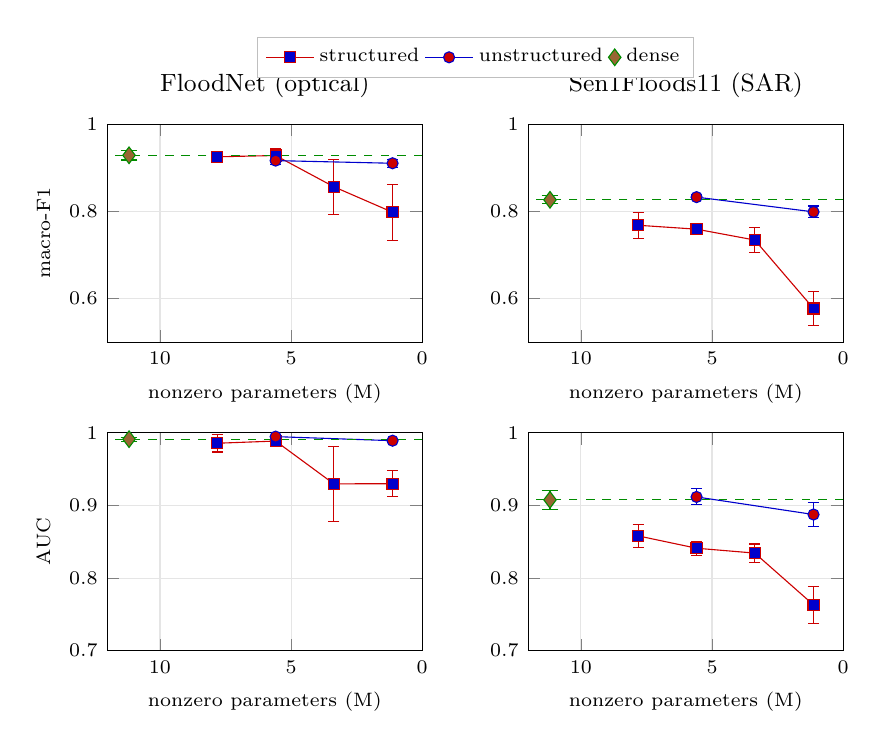
\begin{tikzpicture}
\begin{groupplot}[
  group style={group size=2 by 2, horizontal sep=1.35cm,
               vertical sep=1.15cm},
  width=0.46\textwidth, height=4.35cm,
  x dir=reverse, xmin=0, xmax=12,
  xlabel={nonzero parameters (M)},
  grid=both, grid style={gray!20},
  tick label style={font=\scriptsize},
  label style={font=\scriptsize},
  title style={font=\small},
  legend style={font=\scriptsize, draw=gray!50},
  error bars/y dir=both, error bars/y explicit,
]
% --- (a) FloodNet macro-F1 ---
\nextgroupplot[title={FloodNet (optical)}, ylabel={macro-F1},
               ymin=0.5, ymax=1.0,
               legend to name=sharedlegend, legend columns=3]
\addplot+[mark=square*, color=red!80!black] coordinates {
 (7.82,0.9253) +- (0,0.0117) (5.59,0.9283) +- (0,0.0160)
 (3.37,0.8566) +- (0,0.0630) (1.13,0.7981) +- (0,0.0638)};
\addlegendentry{structured}
\addplot+[mark=*, color=blue!80!black] coordinates {
 (5.59,0.9166) +- (0,0.0097) (1.13,0.9105) +- (0,0.0092)};
\addlegendentry{unstructured}
\addplot+[only marks, mark=diamond*, mark size=3pt,
          color=green!55!black] coordinates {
 (11.18,0.9288) +- (0,0.0107)};
\addlegendentry{dense}
\addplot[dashed, color=green!55!black, domain=0:12] {0.9288};
% --- (b) SAR macro-F1 ---
\nextgroupplot[title={Sen1Floods11 (SAR)}, ymin=0.5, ymax=1.0]
\addplot+[mark=square*, color=red!80!black] coordinates {
 (7.82,0.7683) +- (0,0.0298) (5.59,0.7593) +- (0,0.0062)
 (3.37,0.7344) +- (0,0.0280) (1.13,0.5774) +- (0,0.0382)};
\addplot+[mark=*, color=blue!80!black] coordinates {
 (5.59,0.8328) +- (0,0.0062) (1.13,0.7990) +- (0,0.0134)};
\addplot+[only marks, mark=diamond*, mark size=3pt,
          color=green!55!black] coordinates {
 (11.18,0.8267) +- (0,0.0091)};
\addplot[dashed, color=green!55!black, domain=0:12] {0.8267};
% --- (c) FloodNet AUC ---
\nextgroupplot[ylabel={AUC}, ymin=0.7, ymax=1.0]
\addplot+[mark=square*, color=red!80!black] coordinates {
 (7.82,0.9856) +- (0,0.0121) (5.59,0.9886) +- (0,0.0042)
 (3.37,0.9297) +- (0,0.0515) (1.13,0.9299) +- (0,0.0180)};
\addplot+[mark=*, color=blue!80!black] coordinates {
 (5.59,0.9947) +- (0,0.0016) (1.13,0.9891) +- (0,0.0018)};
\addplot+[only marks, mark=diamond*, mark size=3pt,
          color=green!55!black] coordinates {
 (11.18,0.9912) +- (0,0.0028)};
\addplot[dashed, color=green!55!black, domain=0:12] {0.9912};
% --- (d) SAR AUC ---
\nextgroupplot[ymin=0.7, ymax=1.0]
\addplot+[mark=square*, color=red!80!black] coordinates {
 (7.82,0.8581) +- (0,0.0154) (5.59,0.8411) +- (0,0.0096)
 (3.37,0.8344) +- (0,0.0125) (1.13,0.7631) +- (0,0.0258)};
\addplot+[mark=*, color=blue!80!black] coordinates {
 (5.59,0.9117) +- (0,0.0110) (1.13,0.8875) +- (0,0.0169)};
\addplot+[only marks, mark=diamond*, mark size=3pt,
          color=green!55!black] coordinates {
 (11.18,0.9077) +- (0,0.0131)};
\addplot[dashed, color=green!55!black, domain=0:12] {0.9077};
\end{groupplot}
\node at ($(group c1r1.north east)!0.5!(group c2r1.north west) +
          (0,0.85cm)$) {\pgfplotslegendfromname{sharedlegend}};
\end{tikzpicture}
\caption{ResNet18 under pruning: macro-F1 (top) and AUC (bottom)
vs.\ nonzero parameters, on FloodNet (left) and Sen1Floods11 (right).
Error bars: std over 3 seeds; dashed line: dense baseline. Unstructured
pruning tracks the dense baseline on both datasets down to 1.13M
parameters; structured pruning tracks it on FloodNet up to 50\% but
degrades monotonically on Sen1Floods11 from the first ratio.}
\label{fig:curves}
\end{figure*}

\subsection{ResNet18: Unstructured Compressibility Transfers;
Structured Does Not}
Table~\ref{tab:resnet} and Fig.~\ref{fig:curves} contain the main
result. Under \textbf{unstructured} pruning, ResNet18 is compressible
to 90\% sparsity (1.13M nonzero parameters) at a macro-F1 cost of at
most $0.03$ on \emph{both} datasets: $0.929 \to 0.911$ on FloodNet and
$0.827 \to 0.799$ on Sen1Floods11, with AUC essentially unchanged. On
these two datasets, unstructured compressibility transfers.

Under \textbf{structured} pruning the picture changes. On FloodNet,
filter pruning is free up to 50\% ($0.929 \to 0.928$ macro-F1,
$-0.001$) and only degrades at 70--90\%. On Sen1Floods11 the same
operator costs macro-F1 from the very first ratio: $-0.058$ at 30\%,
$-0.068$ at 50\%, $-0.092$ at 70\%, and $-0.249$ at 90\%, with AUC
falling in step ($0.908 \to 0.763$). The degradation is monotonic,
exceeds seed noise by an order of magnitude at 50\% (std $0.006$), and
has no counterpart on the optical dataset at the same ratios. We state
this as a finding \emph{on these two datasets}: the same structured
pruning protocol that is harmless at 50\% on FloodNet removes capacity
that the Sen1Floods11 task evidently needs.

\subsection{The Learning-Rate Control}
One mundane explanation would be that our fine-tuning recipe (SGD, lr
$0.01$, 50 epochs) is simply mis-tuned for pruned SAR models.
Table~\ref{tab:lrcontrol} tests this with fine-tuning at lr $0.001$.
The lower rate does not recover Sen1Floods11: $0.718$ vs.\ $0.759$ at
50\% (worse), $0.609$ vs.\ $0.577$ at 90\% (marginally better, still
$0.218$ below dense). On FloodNet it is neutral at 50\% and harmful at
90\%. The structured-pruning gap between the two datasets is therefore
not an artifact of the fine-tuning learning rate.

\subsection{VGG-16: An Instability Case}
\begin{table}[t]
\centering
\caption{VGG-16, final-epoch macro-F1 and AUC (mean $\pm$ std, 3
seeds; lr-control row: 2 seeds). $\dagger$: at least one seed
collapsed to a constant predictor (balanced accuracy $0.5$).}
\label{tab:vgg}
\footnotesize
\setlength{\tabcolsep}{2.6pt}
\begin{tabular}{llcc cc}
\toprule
& & \multicolumn{2}{c}{\textbf{FloodNet}} &
\multicolumn{2}{c}{\textbf{Sen1Floods11}}\\
\cmidrule(lr){3-4}\cmidrule(lr){5-6}
\textbf{Method} & \textbf{Ratio} & \textbf{mF1} & \textbf{AUC} &
\textbf{mF1} & \textbf{AUC}\\
\midrule
dense      & 0\%  & .924$\pm$.006 & .990$\pm$.000 & .621$\pm$.262$^\dagger$ & .858$\pm$.003\\
unstruct.  & 50\% & .924$\pm$.006 & .990$\pm$.001 & .601$\pm$.248$^\dagger$ & .849$\pm$.005\\
unstruct.  & 90\% & .943$\pm$.015 & .980$\pm$.020 & .597$\pm$.245$^\dagger$ & .846$\pm$.014\\
struct.    & 30\% & .386$\pm$.199$^\dagger$ & .737$\pm$.035 & .586$\pm$.237$^\dagger$ & .834$\pm$.005\\
struct.    & 50\% & .803$\pm$.076 & .940$\pm$.027 & .519$\pm$.190$^\dagger$ & .788$\pm$.007\\
struct.    & 70\% & .621$\pm$.064 & .675$\pm$.187 & .300$\pm$.070$^\dagger$ & .502$\pm$.225\\
struct.    & 90\% & .230$\pm$.167$^\dagger$ & .500$\pm$.000 & .300$\pm$.070$^\dagger$ & .500$\pm$.000\\
\midrule
str.\ lr .001 & 70\% & .289$\pm$.177$^\dagger$ & .922$\pm$.003 & .325$\pm$.074$^\dagger$ & .700$\pm$.000\\
\bottomrule
\end{tabular}
\end{table}

\begin{table}[t]
\centering
\caption{Per-seed VGG-16 \emph{dense} results on Sen1Floods11
(final epoch). Seed 42 collapses to the constant non-flooded
predictor, yet its AUC remains $0.858$: the learned ranking is intact
and the failure is the final-epoch decision threshold.}
\label{tab:vggperseed}
\footnotesize
\begin{tabular}{lcccc}
\toprule
\textbf{Seed} & \textbf{Acc} & \textbf{Bal.\ Acc} & \textbf{mF1} &
\textbf{AUC}\\
\midrule
42 (failed) & 0.335 & 0.500 & 0.251 & 0.858\\
124         & 0.819 & 0.800 & 0.798 & 0.861\\
2024        & 0.828 & 0.827 & 0.814 & 0.855\\
\bottomrule
\end{tabular}
\end{table}

We report VGG-16 not as a second clean data point but as an
instability case (Table~\ref{tab:vgg}). Three observations.

First, dense VGG-16 training on Sen1Floods11 is itself unreliable:
accuracy is $0.661\pm0.230$ over three seeds.
Table~\ref{tab:vggperseed} breaks this down per seed: seeds 124 and
2024 train normally (macro-F1 $\approx 0.80$), while seed 42 ends at
the constant non-flooded predictor (balanced accuracy $0.500$).
Crucially, the failed seed's AUC is $0.858$ --- indistinguishable from
the healthy seeds. The representation ranks flooded above non-flooded
chips correctly; what fails is the position of the decision boundary
at the final epoch. This is a final-epoch thresholding pathology of a
high-capacity model on 220 training chips, not evidence that VGG-16
cannot encode the SAR task.

Second, structured VGG-16 collapses on \emph{both} datasets (daggered
rows: 90\% on FloodNet, 70--90\% on Sen1Floods11, and sporadically at
30\% on FloodNet), always to a constant predictor with AUC at or near
$0.5$. A layer-level count explains why: our per-layer operator removes
the $\mathrm{round}(r\,n)$ smallest-norm filters from a layer of width
$n$, so at $r=0.9$ the VGG-16 stem retains only 6 of 64 filters
(13/128, 26/256, 51/512 deeper on, 410/4096 in the fully connected
layers). Because VGG-16 is a single serial path with no skip
connections, every prediction must pass through these near-empty
layers, whereas ResNet18's parameter-free identity shortcuts --- which
are never pruned --- preserve an information path around damaged
blocks, which is why ResNet18 degrades gracefully where VGG-16
collapses.

Third, VGG-16 at 90\% \emph{unstructured} on FloodNet reaches
macro-F1 $0.943\pm0.015$ vs.\ dense $0.924\pm0.006$; we note explicitly
that this difference is within seed noise and we do \emph{not} claim
pruning improves VGG-16 --- the supportable statement is that 90\%
unstructured sparsity is cost-free for VGG-16 on FloodNet.

\subsection{Answer to the Title Question}
On these two datasets: compressibility transfers under unstructured
magnitude pruning --- a 90\%-sparse ResNet18 is within $0.03$ macro-F1
of dense on both the optical and the SAR task --- but it does not
transfer under structured filter pruning, where the optical task
tolerates 50\% filter removal at no cost while the SAR task pays
$0.068$ macro-F1 at the same ratio and degrades monotonically
thereafter, robustly to the fine-tuning learning rate. Practically: a
sparsity budget validated on one sensor's data cannot be assumed to
hold for another's, and structured compression in particular should be
re-validated, with balanced metrics and AUC, on every target dataset.

% ------------------------------------------------------------------
\section{Limitations}
\label{sec:limitations}
\textbf{Two datasets, many differences.} FloodNet and Sen1Floods11
differ not only in sensor physics but also in size (398 vs.\ 441
labeled images), spatial resolution ($3000\times4000$ UAV frames vs.\
$512\times512$ 10\,m satellite chips), class imbalance (12.8\% vs.\
66.4\% flooded), scene content and geography, and label provenance
(direct image-level annotation vs.\ labels derived from segmentation
masks via Eq.~\eqref{eq:labelconv}). Our design holds the pipeline
fixed and can therefore attribute the gap to \emph{the dataset}, but
not to sensor modality specifically. All claims in this paper are
scoped to these two datasets; generalizing to ``SAR vs.\ optical''
requires paired acquisitions and more datasets per modality.

\textbf{Three seeds, small evaluation sets.} Mean $\pm$ std over three
seeds distinguishes the large structured-pruning effects (e.g., the
$0.068$ drop at 50\% against std $0.006$) but not fine-grained
differences; evaluation uses 199 images (only ${\sim}25$ flooded) on
FloodNet and
221 chips on Sen1Floods11, so single-image changes are visible in the
metrics. The withheld FloodNet val/test labels force evaluation on a
split of the 398 labeled images.

\textbf{Final-epoch protocol.} Reporting the final epoch avoids
checkpoint cherry-picking but exposes threshold instabilities (the
VGG-16 seed-42 case); a calibration step or threshold selection on a
held-out set would likely remove that failure mode and should
accompany deployments.

\textbf{Label conversion threshold.} Sen1Floods11 image labels depend
on the $\tau=1\%$ rule of Eq.~\eqref{eq:labelconv}; a sensitivity
analysis over $\tau$ is left to future work.

\textbf{Masked rather than physically removed structure.} Pruning is
applied as weight masks; structured channels are zeroed, not excised,
so FLOP reductions are theoretical, and unstructured sparsity yields
no wall-clock speedup without sparse kernels. Neither affects the
accuracy comparison, which is our focus.

\textbf{ImageNet pretraining.} Both backbones start from RGB-pretrained
weights, which is standard but favorable to the optical dataset;
SAR-specific pretraining might shift where structured pruning begins
to hurt.

% ------------------------------------------------------------------
\section{Conclusion}
We asked whether CNN compressibility transfers across sensing
modalities and answered it with a controlled 96-run study on FloodNet
(optical) and Sen1Floods11 (SAR) under a single fixed pipeline. On
these two datasets, unstructured magnitude pruning transfers ---
ResNet18 keeps macro-F1 within $0.03$ of dense at 90\% sparsity on
both --- while structured filter pruning does not: harmless at 50\% on
the optical dataset, it costs $0.068$ macro-F1 on the SAR dataset at
the same ratio, degrades monotonically with ratio, and is not repaired
by a lower fine-tuning learning rate. VGG-16 serves as a cautionary
instability case: seed-level dense failures on SAR that are threshold
rather than representation pathologies (AUC stable at $0.858$), and
structured collapse on both datasets traceable to near-empty layers in
a skip-connection-free architecture. The practical recommendation is
direct: compression choices --- especially structured ones --- should
be re-validated per dataset with balanced accuracy, macro-F1 and AUC
reported together, and sparsity budgets should not be ported across
sensors untested. Future work includes paired optical/SAR
acquisitions to isolate modality, more seeds and datasets,
sensitivity analysis of the label-conversion threshold, and
channel-importance analysis of which filters structured pruning
removes on SAR.

% ------------------------------------------------------------------
\begin{thebibliography}{00}
\bibitem{rahnemoonfar2021floodnet}
M. Rahnemoonfar, T. Chowdhury, A. Sarkar, D. Varshney, M. Yari, and
R. R. Murphy, ``FloodNet: A high resolution aerial imagery dataset for
post flood scene understanding,'' \emph{IEEE Access}, vol.~9, pp.
89644--89654, 2021.

\bibitem{bonafilia2020sen1floods11}
D. Bonafilia, B. Tellman, T. Anderson, and E. Issenberg,
``Sen1Floods11: A georeferenced dataset to train and test deep learning
flood algorithms for Sentinel-1,'' in \emph{Proc. IEEE/CVF Conf.
Comput. Vis. Pattern Recognit. Workshops (CVPRW)}, 2020, pp. 210--211.

\bibitem{khose2021semisupervised}
S. Khose, A. Tiwari, and A. Ghosh, ``Semi-supervised classification and
segmentation on high resolution aerial images,'' in \emph{NeurIPS
Workshop on Tackling Climate Change with Machine Learning}, 2021,
arXiv:2105.08655.

\bibitem{khan2023floodresnet50}
M. A. Khan, N. Ahmed, J. Padela, M. S. Raza, A. Gangopadhyay, J. Wang,
J. Foulds, C. Busart, and R. F. Erbacher, ``Flood-ResNet50: Optimized
deep learning model for efficient flood detection on edge device,'' in
\emph{Proc. IEEE Int. Conf. Mach. Learn. Appl. (ICMLA)}, 2023, pp.
512--519.

\bibitem{han2015learning}
S. Han, J. Pool, J. Tran, and W. J. Dally, ``Learning both weights and
connections for efficient neural networks,'' in \emph{Adv. Neural Inf.
Process. Syst. (NeurIPS)}, 2015, pp. 1135--1143.

\bibitem{li2017pruning}
H. Li, A. Kadav, I. Durdanovic, H. Samet, and H. P. Graf, ``Pruning
filters for efficient ConvNets,'' in \emph{Int. Conf. Learn.
Representations (ICLR)}, 2017.

\bibitem{frankle2019lottery}
J. Frankle and M. Carbin, ``The lottery ticket hypothesis: Finding
sparse, trainable neural networks,'' in \emph{Int. Conf. Learn.
Representations (ICLR)}, 2019.

\bibitem{liu2019rethinking}
Z. Liu, M. Sun, T. Zhou, G. Huang, and T. Darrell, ``Rethinking the
value of network pruning,'' in \emph{Int. Conf. Learn. Representations
(ICLR)}, 2019.

\bibitem{blalock2020state}
D. Blalock, J. J. Gonzalez Ortiz, J. Frankle, and J. Guttag, ``What is
the state of neural network pruning?'' in \emph{Proc. Mach. Learn.
Syst. (MLSys)}, 2020.

\bibitem{he2016resnet}
K. He, X. Zhang, S. Ren, and J. Sun, ``Deep residual learning for image
recognition,'' in \emph{Proc. IEEE Conf. Comput. Vis. Pattern
Recognit. (CVPR)}, 2016, pp. 770--778.

\bibitem{simonyan2015vgg}
K. Simonyan and A. Zisserman, ``Very deep convolutional networks for
large-scale image recognition,'' in \emph{Int. Conf. Learn.
Representations (ICLR)}, 2015.

\bibitem{deng2009imagenet}
J. Deng, W. Dong, R. Socher, L.-J. Li, K. Li, and L. Fei-Fei,
``ImageNet: A large-scale hierarchical image database,'' in \emph{Proc.
IEEE Conf. Comput. Vis. Pattern Recognit. (CVPR)}, 2009, pp. 248--255.

\bibitem{lee2013pseudo}
D.-H. Lee, ``Pseudo-label: The simple and efficient semi-supervised
learning method for deep neural networks,'' in \emph{ICML Workshop on
Challenges in Representation Learning}, 2013.

\end{thebibliography}

\end{document}
